\newcommand{\loga}{logaritamske funkcije}
Logaritamska funkcija uzima broj i vraća potenciju na koju moramo stavitu bazu logaritamske funkcije kako bi dobili argument.
Pronalazimo je u obliku:
\[f(x) = log_ax\;a > 0,\; a \neq 1\]

\subsubsection{Domena i kodomena \loga}
    Domena eksponencijalne funkcija je po definiciji skup \(\mathbb{R^+}\).
    To je intuitivno jasno jer ne možemo naći potenciju negativnog broja.
    Kodomena eksponencijalne funkcije skup \(\mathbb{R}\).

\subsubsection{Graf \loga}
    Specifičnost grafa eksponencijalne funkcije je da uvijek prolazi kroz točku \((0, 1)\).
    Mijenjamo li bazu \(a\), mijenja se \emph{brzina} rasta. Dodavanjem slobodnog koeficijnta mjenjanmo odsječak na y-osi.
    \begin{figure}[ht]
        \centering
        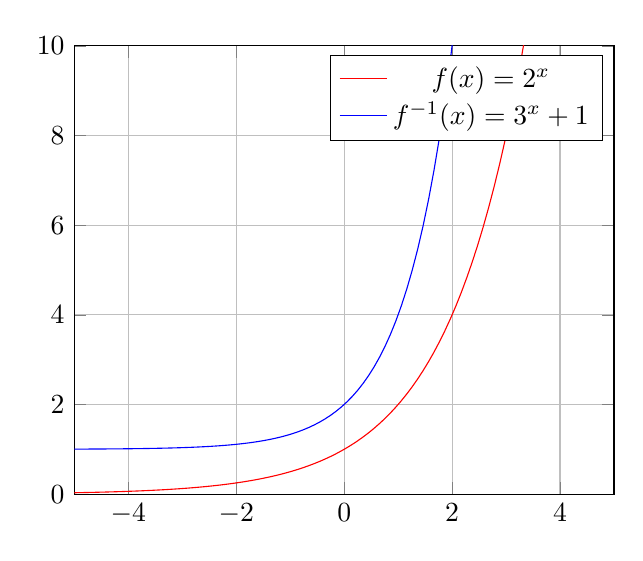
\begin{tikzpicture}
            \begin{axis}[
                grid=major,
                ymin=0,
                ymax=10,
                xmin=-5,
                xmax=5,
            ]
                \addplot[
                    color = red,
                    samples = 100
                ]{2^x};
                \addlegendentry{\(f(x) = 2^x\)}
                \addplot[
                    color = blue,
                    samples = 100
                ]{3^x + 1};
                \addlegendentry{\(f^{-1}(x) = 3^x + 1\)}
            \end{axis}
        \end{tikzpicture}
        \caption{Grafovi eksponencijalne funkcije s različitim parametrima}
        \label{fig:template}
    \end{figure}
\subsubsection{Nultočke i točke u kojima graf sječe y-os \loga}
\subsubsection{Parnost i neparnost \loga}
\subsubsection{Periodičnost \loga}
\subsubsection{Monotonost \loga}
\subsubsection{Omeđenost \loga}
\subsubsection{Injektivnost i surjektivnost \loga}
\subsubsection{Inverz \loga}
Inverz eksponencijalne funkcije je logaritamska funkcija.
    \begin{figure}[ht]
        \centering
        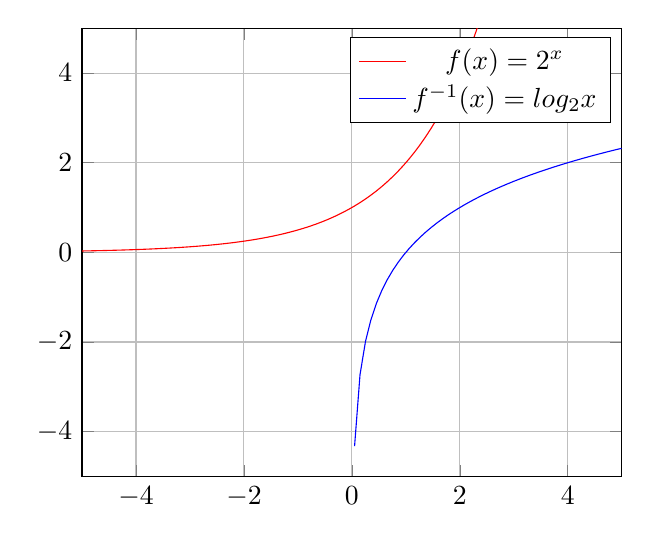
\begin{tikzpicture}
            \begin{axis}[
                grid=major,
                ymin=-5,
                ymax=5,
                xmin=-5,
                xmax=5,
            ]
                \addplot[
                    color = red,
                    samples = 100
                ]{2^x};
                \addlegendentry{\(f(x) = 2^x\)}
                \addplot[
                    color = blue,
                    samples = 100
                ]{log2(x)};
                \addlegendentry{\(f^{-1}(x) = log_2x\)}
            \end{axis}
        \end{tikzpicture}
        \caption{Grafovi funkcije i njenzinog inverzna}
        \label{fig:template}
    \end{figure}
    \\